\documentclass[border=10pt]{standalone}
\usepackage{tikz}
\usepackage{amsmath}
\usetikzlibrary{arrows.meta, calc}

% ── palette ──────────────────────────────────────────────────────────────────
\definecolor{cblue}{RGB}{191,215,237}
\definecolor{cblueedge}{RGB}{43,108,176}
\definecolor{cgray}{RGB}{214,214,214}
\definecolor{camber}{RGB}{255,208,128}
\definecolor{camberedge}{RGB}{192,90,0}
\definecolor{cgreen}{RGB}{184,224,184}
\definecolor{cleg}{RGB}{250,250,250}

\tikzset{
  iboxL/.style={   % left-branch input (blue)
    draw=cblueedge, fill=cblue, rounded corners=3pt,
    minimum width=1.85cm, minimum height=0.52cm,
    align=center, font=\small, inner sep=4pt, line width=0.8pt
  },
  iboxR/.style={   % right-branch input (gray, no object colour)
    draw=gray!75, fill=cgray, rounded corners=3pt,
    minimum width=1.85cm, minimum height=0.52cm,
    align=center, font=\small, inner sep=4pt, line width=0.8pt
  },
  abox/.style={    % analytical / concat
    draw=gray!75!black, fill=gray!13, rounded corners=3pt,
    minimum width=2.6cm, minimum height=0.58cm,
    align=center, font=\small, inner sep=4pt, line width=0.8pt
  },
  mbox/.style={    % MLP dense layer (amber)
    draw=camberedge, fill=camber, rounded corners=3pt,
    minimum width=2.6cm, minimum height=0.52cm,
    align=center, font=\small, inner sep=4pt, line width=0.8pt
  },
  obox/.style={    % output
    draw=black!75, fill=cgreen, rounded corners=4pt,
    minimum width=10.0cm, minimum height=0.55cm,
    align=center, inner sep=5pt, line width=0.9pt
  },
  tbox/.style={    % training step box
    draw=gray!50, fill=gray!7, rounded corners=3pt,
    minimum width=3.0cm, minimum height=0.62cm,
    align=center, font=\small, inner sep=3pt, line width=0.65pt
  },
  larr/.style={-{Stealth[length=4pt]}, line width=0.80pt, color=cblueedge},
  rarr/.style={-{Stealth[length=4pt]}, line width=0.80pt, color=camberedge},
  darr/.style={-{Stealth[length=4pt]}, line width=0.80pt, color=gray!65!black},
  barr/.style={-{Stealth[length=5pt]}, line width=1.05pt, color=black!70},
  tarr/.style={-{Stealth[length=3.5pt]}, line width=0.70pt, color=gray!55},
}

% ── coordinate layout (all in cm) ────────────────────────────────────────────
% Left group:  3 inputs at x = 0.0, 2.2, 4.4   → M3CB centre x = 2.2
% Right group: 4 inputs at x = 7.4, 9.6, 11.8, 14.0  → φ centre x = 10.7
% ⊕ / output centred at x = 6.45  (midpoint of 2.2 and 10.7)

\begin{document}
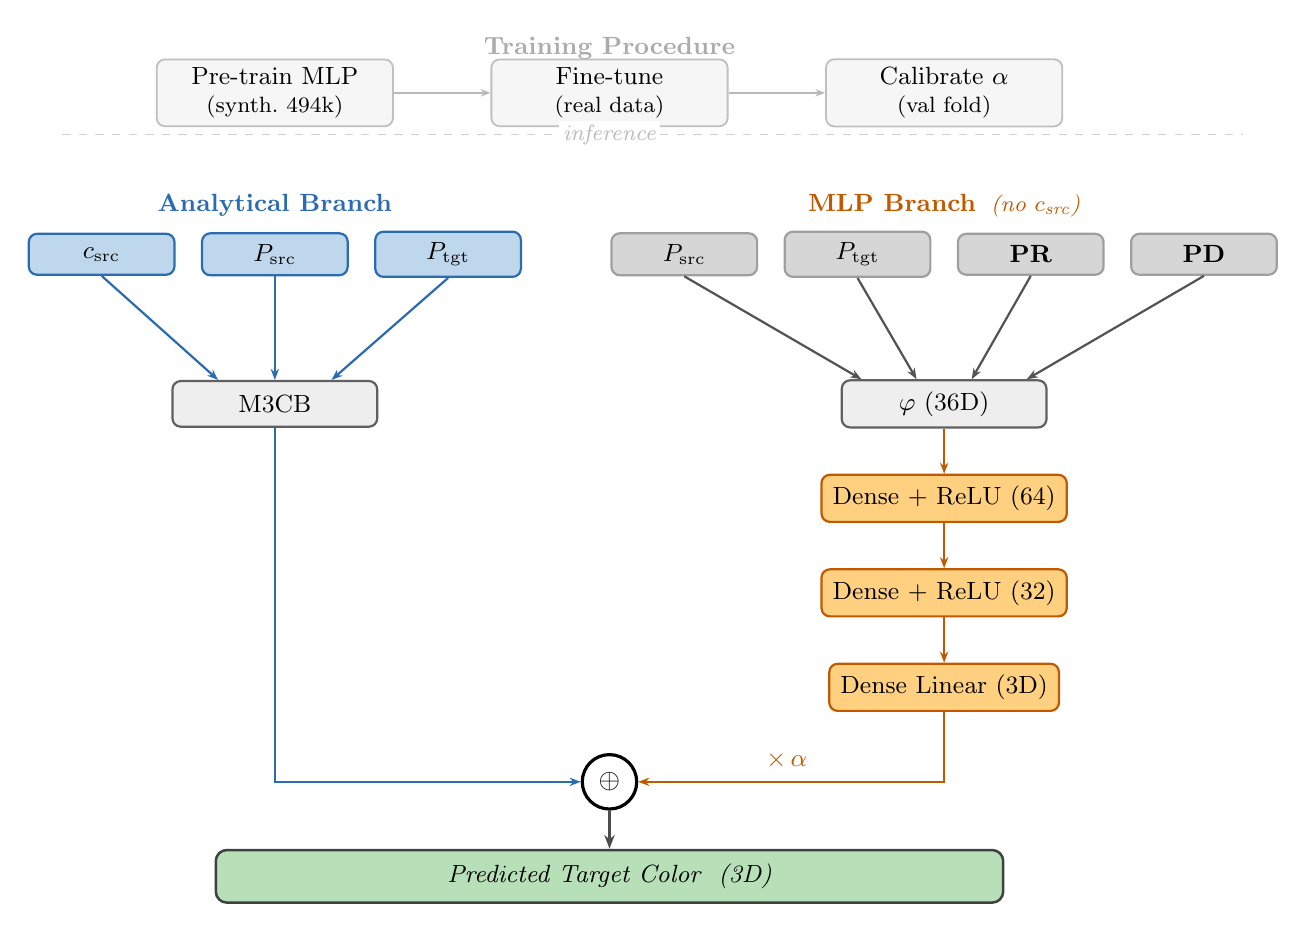
\begin{tikzpicture}

%% ─── TRAINING PROCEDURE (top strip) ──────────────────────────────────────────
\node[font=\small\bfseries, color=gray!65] at (6.45, 2.62)
  {Training Procedure};

\node[tbox] (t1) at ( 2.20, 2.05) {Pre-train MLP\\[-1pt]{\footnotesize(synth.\ 494k)}};
\node[tbox] (t2) at ( 6.45, 2.05) {Fine-tune\\[-1pt]{\footnotesize(real data)}};
\node[tbox] (t3) at (10.70, 2.05) {Calibrate $\alpha$\\[-1pt]{\footnotesize(val fold)}};

\draw[tarr] (t1.east) -- (t2.west);
\draw[tarr] (t2.east) -- (t3.west);

% Dashed separator with centred label
\draw[dashed, gray!38, line width=0.60pt] (-0.5, 1.52) -- (14.5, 1.52);
\node[font=\footnotesize\itshape, color=gray!55, fill=white, inner sep=1.5pt]
  at (6.45, 1.52) {inference};

%% ─── LEFT: Analytical branch inputs (horizontal row) ─────────────────────────
\node[iboxL] (csrc)  at ( 0.0, 0) {$c_{\text{src}}$};
\node[iboxL] (psrc1) at ( 2.2, 0) {$P_{\text{src}}$};
\node[iboxL] (ptgt1) at ( 4.4, 0) {$P_{\text{tgt}}$};

\node[font=\small\bfseries, color=cblueedge] at (2.2, 0.62)
  {Analytical Branch};

%% M3CB
\node[abox] (m3cb) at (2.2, -1.90) {M3CB};

% Fan arrows: each input at a different x → naturally diagonal into M3CB
\draw[larr] (csrc.south)  -- ($(m3cb.north) + (-0.72cm, 0)$);
\draw[larr] (psrc1.south) --   (m3cb.north);
\draw[larr] (ptgt1.south) -- ($(m3cb.north) + ( 0.72cm, 0)$);

%% ─── RIGHT: MLP branch inputs (horizontal row) ───────────────────────────────
\node[iboxR] (psrc2) at ( 7.4, 0) {$P_{\text{src}}$};
\node[iboxR] (ptgt2) at ( 9.6, 0) {$P_{\text{tgt}}$};
\node[iboxR] (ratio) at (11.8, 0) {\textbf{PR}};
\node[iboxR] (diffs) at (14.0, 0) {\textbf{PD}};

\node[font=\small\bfseries, color=camberedge] at (10.7, 0.62)
  {MLP Branch\enspace{\normalfont\footnotesize\itshape (no $c_{\text{src}}$)}};

%% φ feature
\node[abox] (phi) at (10.7, -1.90) {$\varphi$ \small(36D)};

% Fan arrows from each right input → different offsets on φ top
\draw[darr] (psrc2.south) -- ($(phi.north) + (-1.05cm, 0)$);
\draw[darr] (ptgt2.south) -- ($(phi.north) + (-0.35cm, 0)$);
\draw[darr] (ratio.south)  -- ($(phi.north) + ( 0.35cm, 0)$);
\draw[darr] (diffs.south)  -- ($(phi.north) + ( 1.05cm, 0)$);

%% MLP dense layers
\node[mbox] (d64)    at (10.7, -3.10) {Dense + ReLU (64)};
\node[mbox] (d32)    at (10.7, -4.30) {Dense + ReLU (32)};
\node[mbox] (linear) at (10.7, -5.50) {Dense Linear (3D)};

\draw[rarr] (phi.south) -- (d64.north);
\draw[rarr] (d64.south) -- (d32.north);
\draw[rarr] (d32.south) -- (linear.north);

%% ─── ⊕ combiner ──────────────────────────────────────────────────────────────
\node[circle, draw=black, fill=white, line width=1.15pt,
      minimum size=0.66cm, font=\normalsize\bfseries]
  (comb) at (6.45, -6.70) {$\oplus$};

% Elbow routes: each branch goes down then horizontal to ⊕
\draw[larr, line width=0.90pt] (m3cb.south)   |- (comb.west);
\draw[rarr, line width=0.90pt] (linear.south) |- (comb.east);

% α label above the right horizontal segment
\node[font=\small\bfseries, color=camberedge] at (8.70, -6.42)
  {${\times}\,\alpha$};

%% ─── Output ──────────────────────────────────────────────────────────────────
\node[obox] (out) at (6.45, -7.90) {%
  {\small\itshape Predicted Target Color \ (3D)}%
};
\draw[barr] (comb.south) -- (out.north);

\end{tikzpicture}
\end{document}
